\begin{figure*}[t]
    \centering
    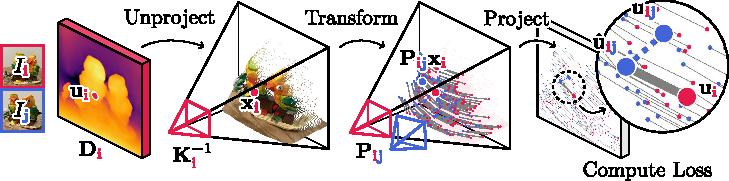
\includegraphics[width=\linewidth,]{figures/loss/fig_loss_pdf.pdf}
    \caption{\textbf{Camera-Induced Flow Loss.} To use a known correspondence $\pixcoord_{ij}$ to compute a loss $\loss$, we unproject $\pixcoord_i$ using the corresponding depth map $\depth_i$ and camera intrinsics $\textbf{K}_i$, transform the resulting point $\pixcoordx_i$ via the relative pose $\mathbf{P}_{ij}$, reproject the transformed point to yield $\hat{\pixcoord}_{ij}$, and finally compute $\loss = \|\hat{\pixcoord}_{ij} - \pixcoord_{ij}\|$.}
    \label{fig:loss}
    \vspace{-10pt}
\end{figure*}
